\section{Layouts for a Superconducting QPU}
\label{sub:ancilla_layouts}

% Sec. IV of the restructured sim version (2026-11-19; style: jpw-review/sim/style-snap.md; outline: jpw-review/sim/outline-II-IV.md). Replaces the former Sec. 2.4 ("method - layouts.tex", kept unused). The two-ancilla layout is the square-lattice layout chosen by the user on 2026-11-17, the one-ancilla round is the five-moment round chosen on 2026-11-19, and panel (a) shows IQM Garnet (2026-11-18); run folders and sources: jpw-review/sim/qlib_new.py and paper-rework/a1-layout-figure/HANDOFF-B.md.
Let us now turn to the hardware. A layout of the code on a QPU places the data and ancilla qutrits on the transmons of a chip and fixes the couplings that the circuits use. Besides the $q_2$--$q_3$ coupling that the logical gates need (\autoref{sub:code}) and the ancillas and couplings of the check rounds (\autoref{sub:lrbd_measures}), a layout with check rounds needs a check round that is safe against single faults: no single fault in a round may cause a logical error that this round and the next both miss. \autoref{fig:ancilla_layouts} shows terminal postselection and two layouts with check rounds that meet these requirements, and \autoref{tab:layouts} lists what each of them uses. In \autoref{sub:layout_terminal} we place terminal postselection on five transmons of an existing chip, in \autoref{sub:layout_one} we give each stabilizer its own ancilla next to its three data qutrits, at the price of one long-range coupling, and show that a square lattice cannot provide both, and in \autoref{sub:layout_two} we keep to a square lattice by letting the data qutrits take part in the check round.

\begin{figure*}[tp]
  % from paper-rework/a1-layout-figure/ancilla-layouts-B.pdf, caption-layout-B.tex part 2 (restructure 2026-11-19)
  \centering
  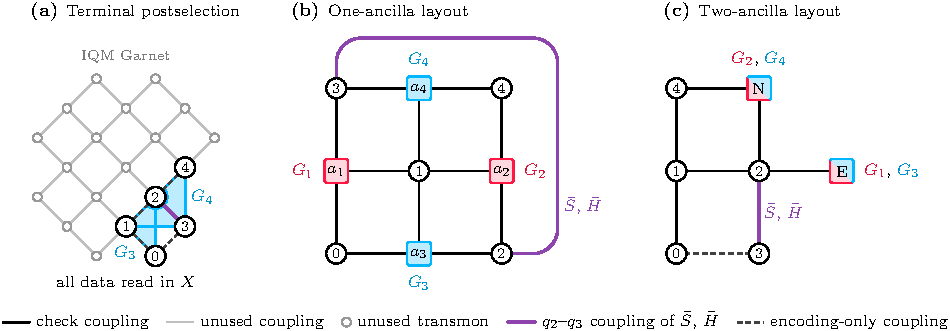
\includegraphics{figures/layouts-three.pdf}% drawn at final size
  \caption{Qutrits and couplings of the $[[5,1,2]]_3$ code in terminal postselection (a) and in the one-ancilla (b) and two-ancilla (c) layouts, with each coupling marked by its use in the stabilizer measurements, the logical gates or the encoding circuit. Circles with an index are data qutrits, small circles are unused transmons, and squares are ancillas. Red marks the $Z$-type stabilizers $G_1$, $G_2$ and blue the $X$-type $G_3$, $G_4$ (Eqs.~\eqref{eq:s1} and~\eqref{eq:s4}), and the label beside an ancilla names the stabilizers it measures in each check round. Dashed couplings are used only by the encoding circuit.
(a)~Terminal postselection on IQM's Garnet QPU, whose 20 transmons sit on a square lattice with 30 couplings between nearest neighbors~\cite{IQM240812433}. Drawn in the orientation of IQM's device map, with QB1 at the bottom, the transmons QB1, QB4, QB5, QB2 and QB6 hold $q_0, \dots, q_4$, respectively. The dashed couplings are the four that its encoding circuit uses (\autoref{fig:encoding_circuit}(a)). No ancillas are used, and the final $X$-basis readout of all data qutrits gives $G_3$ and $G_4$ (shaded; their blue outlines are not couplings, and that of $G_4$ bends around $q_2$).
(b)~One-ancilla layout on the conventional surface-code grid, with $q_1$ at the center. Ancilla $a_j$ neighbors the three data qutrits of $G_j$, and the two-qutrit gates of $\bar H$ and $\bar S$ (Eqs.~\eqref{eq:logical_H} and~\eqref{eq:logical_HS}) need a long-range coupling between $q_2$ and $q_3$. The encoding circuit of this layout (\autoref{fig:encoding_circuit}(b)) uses only check couplings, so this panel has no dashed coupling.
(c)~Two-ancilla layout: the ancillas N and E and eight couplings, all between nearest neighbors of a square lattice. N measures $G_2$ and then $G_4$, and E measures $G_1$ and then $G_3$, so each of their squares carries both colors. Neither ancilla is next to all three data qutrits of these stabilizers, so the extraction circuits (\autoref{fig:extraction_circuits}(e)--(h)) also apply SUM gates and their inverses between data qutrits, on $q_0$--$q_1$, $q_1$--$q_2$, $q_1$--$q_4$ and $q_2$--$q_3$, the coupling that also carries the two-qutrit gates of $\bar H$ and $\bar S$. The encoding circuit of this layout (\autoref{fig:encoding_circuit}(c)) uses the dashed coupling $q_0$--$q_3$ and three solid ones.}
  \label{fig:ancilla_layouts}
\end{figure*}


\begin{table}[tp]% single-column
  \centering
  \begin{tabular}{lccccc}
    \hline\hline
     & & & two-qutrit & gate & \\
     & qutrits & couplings & gates & moments & readouts \\
    \hline
    terminal & 5 & 5 & -- & -- & -- \\
    one-ancilla & 9 & 13 & 12 & 5 & 4 \\
    two-ancilla & 7 & 8 & 24 & 19 & 4 \\
    \hline\hline
  \end{tabular}
  \caption{Resources of terminal postselection and of the one-ancilla and two-ancilla layouts of \autoref{fig:ancilla_layouts}: the qutrits, the couplings used by any circuit (encoding, logical gates, check rounds), and the two-qutrit gates, gate moments and ancilla readouts of one check round. A gate moment is a set of gates on disjoint qutrits that run in parallel; a check round also has one reset moment and one readout moment in the one-ancilla layout, and one reset and two readout moments in the two-ancilla layout.}
  \label{tab:layouts}
\end{table}

\subsection{Terminal Postselection on Five Transmons}
\label{sub:layout_terminal}

\autoref{fig:ancilla_layouts}(a) places terminal postselection on IQM's Garnet QPU~\cite{IQM240812433}: the five data qutrits occupy five transmons chosen so that the four couplings of the encoding circuit and the coupling $q_2$--$q_3$ of the logical gates, all five couplings that its circuits use (\autoref{tab:layouts}), are couplings of the chip.

\subsection{One-Ancilla Layout}
\label{sub:layout_one}

The most direct way to supply the ancillas of uniform-interval postselection gives each stabilizer its own ancilla next to its three data qutrits. On the conventional surface-code grid, one data qutrit at the center of a square and four at its corners, each ancilla can neighbor all three data qutrits of its stabilizer when $q_1$, the one qutrit in all four generators, sits at the center (\autoref{fig:ancilla_layouts}(b)). Every stabilizer then acts on the center and two adjacent corners, so the ancilla $a_j$ on the site between them measures $G_j$ with one SUM gate or its inverse per data qutrit, between $H$ and $H^{-1}$ for the $X$-type generators (\autoref{fig:extraction_circuits}(a)--(d)). The round needs no gate between data qutrits, and \autoref{tab:layouts} gives its gates and its length. Of all orders of these gates that measure the four syndromes correctly, we use one with the smallest coefficient of $p^2$ in the logical error rate per round when check rounds run back to back and every round is postselected under both noise models of \autoref{sub:noise_models}, and the round is safe against single faults (\appref{app:rounds-one-ancilla}). In this layout, however, $q_2$ and $q_3$ sit at opposite corners, so the two-qutrit gates of $\bar H$ and $\bar S$ need a long-range coupling.

One may ask whether a square lattice, the connectivity of Garnet, can give each stabilizer an ancilla next to its three data qutrits and still couple $q_2$ and $q_3$. It cannot. A square lattice is bipartite, so all neighbors of a site belong to the same sublattice. An ancilla next to the data qutrits of $G_3$ puts $q_0$, $q_1$ and $q_2$ on one sublattice, and an ancilla next to those of $G_1$ puts $q_0$, $q_1$ and $q_3$ on one sublattice. Then $q_2$ and $q_3$ share a sublattice, and no coupling of the lattice joins them. The same argument with $G_2$ and $G_4$ puts $q_2$ and $q_3$ on one sublattice again. On a square lattice at least one of $G_1$ and $G_3$, and at least one of $G_2$ and $G_4$, must therefore be measured by an ancilla that does not touch all of its data qutrits, and the missing values must reach that ancilla through other gates.

\subsection{Two-Ancilla Layout}
\label{sub:layout_two}

The two-ancilla layout measures all four stabilizers in this way, with two ancillas (\autoref{fig:ancilla_layouts}(c)). The ancillas are named N and E after their positions in \autoref{fig:ancilla_layouts}(c); in each check round N measures $G_2$ and then $G_4$, and E measures $G_1$ and then $G_3$. The key idea is that a gate between two data qutrits, a data gate, can move a value from a qutrit that the ancilla does not touch onto one that it does, and can be undone afterwards. Let $z_j$ be the computational-basis value of $q_j$. To measure $G_2 = Z_1 Z_2 Z_4^{-1}$, for example, N first adds $z_2$, the value of its neighbor $q_2$. A data gate then sets $q_4$ to $z_4 - z_1$, N subtracts this value, and the data gate is undone, so that N holds $z_1 + z_2 - z_4$, the syndrome of $G_2$ (\autoref{fig:extraction_circuits}(e)). The $X$-type generators are collected in the same way between $H$ and $H^{-1}$ (\autoref{fig:extraction_circuits}(g), (h)). N and E are reset at the start of the round and read out after each of their two measurements, without a reset in between, so the second readout of each is its first readout plus the second syndrome, modulo three.

This design has a price: 16 of the 24 two-qutrit gates of the round are data gates, the round has almost four times as many gate moments as the one-ancilla round (\autoref{tab:layouts}), and a fault on a data gate can reach two data qutrits. The gates are nevertheless ordered so that the round is safe against single faults in the sense of the opening of this section (\appref{app:rounds-relay}). In return for the longer round, the two-ancilla layout fits on the square lattice of Garnet, in 48 ways of mapping its seven qutrits onto transmons such that all eight of its couplings are couplings of the chip.
